%\documentclass{beamer}
\documentclass[handout,xcolor=pdftex,dvipsnames,table]{beamer} % for handouts

\usecolortheme[RGB={0,0,144}]{structure}
\usetheme{AnnArbor}
\useoutertheme{infolines}

\usepackage{hyperref, amsmath}
\usepackage{tikz, caption}
\usepackage{verbatim,xmpmulti,color,multicol,multirow,graphicx,natbib,undertilde}
\setlength{\unitlength}{\textwidth}  % measure in textwidths

\graphicspath{{/Users/Danny/Documents/"UCSB - Research"/Thesis/graphs/},
{/Users/Danny/Documents/"UCSB - Research"/Thesis/graphs/fmri/}
}

\def\newblock{\hskip .11em plus .33em minus .07em}

%\usepackage{beamerthemesplit}
\setbeamertemplate{navigation symbols}{}
\setbeamercolor{alerted text}{fg=red}
\setbeamertemplate{block body theorem}{bg=orange}
\setkeys{Gin}{width=0.6\textwidth}

\title[SMC applications: epidemics and fMRI]{Sequential Monte Carlo methods: applications to disease surveillance and fMRI data}
\subtitle{Dissertation Defense}
\author[Daniel M. Sheinson]{Daniel M. Sheinson \\ \ \\ Committee: Jarad Niemi (co-chair), Wendy Meiring (co-chair), \\ Greg Ashby, John Hsu}
\institute[UCSB]{University of California, Santa Barbara}
\date{August 15, 2014}

\begin{document}

\frame{\titlepage}

\frame{\frametitle{Outline} \pause
Introduction / Motivation \\ \pause
State-space models
\begin{itemize}
\item Dynamic linear models
\item Sequential estimation
\end{itemize} \pause
Sequential Monte Carlo methods
\begin{itemize}
\item particle filters
\item model comparison
\end{itemize} \pause
Analysis of fMRI data \pause
\begin{itemize}
\item standard approaches \pause
\item SMC model comparison
\end{itemize}
}

\section{Introduction / Motivation \label{sec:def:intro}}

\frame{\frametitle{Sequential data} \pause
observations collected over time \\ \pause
\begin{itemize}
\item nonlinear \pause
\item temporally autocorrelated \pause
\end{itemize}
Syndromic surveillance \\ \pause
\begin{itemize}
\item on-line epidemic tracking \pause
\item sequential analysis \pause
\end{itemize}
Functional magnetic resonance imaging (fMRI) \pause
\begin{itemize}
\item accurately model physiological response to neural activation \pause
\item model comparison strategy \pause
\end{itemize}
Sequential Monte Carlo methods \\ \pause
\begin{itemize}
\item sequential estimation \pause
\item direct way to compare models
\end{itemize}
}

\section{State-space models \label{sec:def:models}}

\frame{\frametitle{State-space models} \pause
\begin{itemize}
\item frequently used to model biological data \pause
\item simultaneously model observed and unobserved processes \pause
\end{itemize}
Governed by two equations:
\begin{enumerate}
\item state equation \pause
\begin{itemize}
\item evolution of the latent, unobserved state over time
\end{itemize} \pause
\item observation equation \pause
\begin{itemize}
\item dependence of observations on the unobserved state
\end{itemize}
\end{enumerate}
}

\frame{\frametitle{State-space models}
Notation \pause
\begin{itemize}
\item $x_t$ - unobserved state vector at time $t$, $t=0,1,2,\ldots,T$ \pause
\item $y_t$ - observed data vector at time $t$, $t=1,2,\ldots,T$ \pause
\item $\theta$ - vector of unknown, fixed parameters \pause
\item $y_{1:t}$ - collection of vectors $y_1,\ldots,y_t$ \pause
\item $p(x_t|x_{t-1},\theta)$ - state transition density (state equation) \pause
\item $p(y_t|x_t,\theta)$ - conditional likelihood (observation equation) \pause
\item $(y_t \perp y_{1:t-1},y_{t+1:T}) | x_t,\theta$ and $(x_t \perp x_{1:t-2},y_{1:t-1}) | x_{t-1},\theta$ \pause
\item $p(x_0,\theta)$ - prior distribution on initial state and fixed parameters \pause
\end{itemize}
\begin{figure}[ht]
\centering
%\caption*{Dependence structure of state-space models}
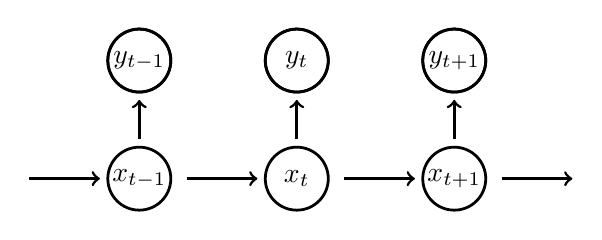
\begin{tikzpicture}[line width=1pt]
\foreach \x in {1,...,3} \draw (3+2*\x,0) circle (0.4cm);
\foreach \x in {1,...,3} \draw (3+2*\x,1.5) circle (0.4cm);
\foreach \x in {1,...,3} \draw (3+2*\x,1.5) circle (0.4cm);
\foreach \x in {1,...,3} \draw [<-] (3+2*\x, 1) -- (3+2*\x,.5);
\foreach \x in {1,...,4} \draw [->] (3+2*\x-1.4, 0) -- (3+2*\x-.5,0);
\draw (3+2*1,0) node {$x_{t-1}$};
\draw (3+2*2,0) node {$x_{t}$};
\draw (3+2*3,0) node {$x_{t+1}$};
\draw (3+2*1,1.5) node {$y_{t-1}$};
\draw (3+2*2,1.5) node {$y_{t}$};
\draw (3+2*3,1.5) node {$y_{t+1}$};
\end{tikzpicture}
\end{figure}
}

%\frame{\frametitle{State-space model of an epidemic} \pause
%Modeling disease transmission: \pause
%\begin{itemize}
%\item SIR model \pause
%\item keep track of \% of population susceptible ($s_t$), infected ($i_t$), and recovered ($r_t$) at each day $t = 0,1,2,\ldots,T$ \pause
%\item fixed population size $P$ \pause
%\item $s_t + i_t + r_t = 1$ \pause
%\item $x_t = (s_t,i_t)$ - unobserved state of the epidemic at day $t$ \pause
%\item fixed parameters $\beta > 0$, $\gamma > 0$, and $\nu > 0$: \pause
%\item $\beta =$ rate of spread \pause
%\item $\gamma =$ recovery time from infection \pause
%\item $\nu =$ population mixing intensity \pause
%\item $\theta = (\beta, \gamma, \nu)'$
%\end{itemize}
%}
%
%\frame{\frametitle{State-space model of an epidemic}
%State equation: \pause
%\[x_{t+1}\left|x_t,\theta\right. \sim \mbox{N}_\Omega\left(f(x_t,\theta),Q(\theta)\right),\]
%where
%\[f(x_t,\theta) = \left(
%\begin{array}{c}
%s_t - \beta i_ts^\nu_t \phantom{- \gamma i_t}\,\, \\
%i_t +  \beta i_ts^\nu_t - \gamma i_t
%\end{array}
%\right),
%\qquad
%Q(\theta) = \frac{\beta}{P^2} \left(
%\begin{array}{ccccc}
%1 & -1 \\
%-1 & 1 + \gamma/\beta
%\end{array}
%\right),\]
%$\Omega = \{(s_t,i_t): s_t \ge 0, i_t \ge 0, s_t + i_t \le 1\}$, and \\ \pause
%$p(x_0,\theta) = p(i_0)\delta_{1-i_0}(s_0)p(\theta)$ with $i_0 \sim \mbox{N}_{[0,1]}(0.002,0.0005^2)$ \pause
%\begin{itemize}
%\item \citet{skvortsov2012monitoring,sheinson:niemi:meiring:epidtrack:2014} \pause
%\item \citet{herwaarden1995stochepid,dangerfield2009stochepid,anderson2004sars}
%\end{itemize}
%}
%
%\frame{\frametitle{State-space model of an epidemic}
%\begin{itemize}
%\item $R_0 = \frac{\beta}{\gamma}$ - basic reproductive number \pause
%\item seasonal flu - $R_0 \approx 1.5$, polio - $R_0 \approx 5$, chicken pox - $R_0 \approx 10$
%\end{itemize} \pause
%\includegraphics[width=0.45\textwidth]{sircurves1} \pause
%\includegraphics[width=0.45\textwidth]{sircurves2}
%}
%
%\frame{\frametitle{State-space model of an epidemic}
%Observation equation: \pause
%\begin{itemize}
%\item observe syndromic data from $L$ streams \pause
%\item $y_{l,t}$ - observed data from stream $l$ at day $t$ \pause
%\item e.g. counts of flu-related internet search queries, emergency room visits, etc. \pause
%\item $y_t = (y_{1,t},y_{2,t},\ldots,y_{L,t})'$ be observed data at day $t$, $t=1,2,\ldots,T$ \pause
%\item assume a stochastic power-law relationship between $\log y_t$ and $i_t$, i.e.
%\[\log y_{l,t} |x_t,\theta \sim \mbox{N}\left(b_li_t^{\varsigma_l}+\eta_l,\sigma_l^2\right)\] \pause
%\item \citet{Gins:Mohe:Pate:Bram:Smol:Bril:dete:2009}, \citet{skvortsov2012monitoring} \pause
%\item initially assume $L = 4$ and $\eta_l$, $b_l$, $\varsigma_l$, and $\sigma_l$ known for all $l$ \pause
%\item extended analysis: $L = 1$ and $\theta = (\beta,\gamma,\nu,b,\varsigma,\sigma,\eta)'$
%\end{itemize}
%}

\subsection{Dynamic linear models}

\frame{\frametitle{Dynamic linear models (DLMs)} \pause
\begin{align*}
\mbox{obs. eqn.:  } & y_t = U_t\beta + F_tx_t + v_t, \quad & v_t &\stackrel{iid}{\sim} \mbox{N}(0,V) \\ \pause
\mbox{state eqn.:  } & x_t = Gx_{t-1} + w_t, \quad & w_t &\stackrel{iid}{\sim} \mbox{N}(0,W) \\ \pause
\mbox{prior:  } & x_0 \sim \mbox{N}(m_0, C_0) \quad & &  \pause
\end{align*}
\begin{align*}
y_t:& \ q \times 1 & U_t:& \ q \times d & \beta:& \ d \times 1 & & \\ \pause
F_t:& \ q \times p & x_t:& \ p \times 1 & v_t:& \ q \times 1 & V:& \ q \times q \\ \pause
G:& \ p \times p & W:& \ p \times p & m_0:& \ p \times 1 & C_0:& \ p \times p \pause
\end{align*}
\begin{itemize}
\item $v_s \perp w_s'$ for all $s \ne s'$ \pause
\item assume univariate $y_t$, i.e. $q = 1$ \pause
\item $G$, $V$, $W$, $C_0$, and $\beta$ could contain unknown fixed parameters
\end{itemize}
}

\frame{\frametitle{First-order DLM with common variance factor} \pause
Let $F_t = G = 1$, $p = 1$, $V = \theta$, and $W = \theta\lambda$ \pause
\begin{align*}
y_t &\sim \mbox{N}(x_t, \theta) \\
x_t &\sim \mbox{N}(x_{t-1}, \theta\lambda)
\end{align*} \pause
\begin{itemize}
\item prior: $x_0|\theta \sim \mbox{N}(0, \theta) \quad \theta \sim \mbox{IG}(a_0,b_0)$ \pause
\item $\theta$ - unknown common state and observation variance factor \pause
\item $\lambda$ - signal-to-noise ratio, assumed known \pause
\item $a_0$ and $b_0$ assumed known
\end{itemize}
}

\frame{\frametitle{Regression with ARMA errors} \pause
\begin{align*}
y_t &= U_t\beta + x_t \\ \pause
x_t &= \phi_1x_{t-1} + \cdots + \phi_Px_{t-P} + \epsilon_t + \gamma_1\epsilon_{t-1} + \cdots + \gamma_Q\epsilon_{t-Q} \\ \pause
\epsilon_j &\stackrel{iid}{\sim} \mbox{N}(0,\sigma^2), \ j \ge 0 \pause
\end{align*}
\[
\begin{array}{ll}
x_t &= (x_{t,1} ,x_{t,2}, \ldots, x_{t,m})' \\
m &= \mbox{max}(P,Q+1) \\ \pause
F_t &= (1,0,\ldots,0)_{1\times m} \\ \pause
v_t &= 0 \\ \pause
W &= \sigma^2ee' \\
e &= (1, \gamma_1, \ldots, \gamma_{m-1})' \\ \pause
\phi_s &= 0, \ s > P \\ \pause
\gamma_r &= 0, \ r > Q \pause
\end{array} \quad
G = \left(
 \begin{array}{ccccc}
 \phi_1 & \vdots \\
 \phi_2 & \vdots \\
 \phi_3 & \vdots && I_{m-1} \\
 \vdots & \vdots \\
 \cdots & \cdots & \cdots & \cdots & \cdots \\
 \phi_m &\vdots & 0 & \cdots & 0
 \end{array}
\right)\] \pause
%$\phi_s = 0$ for $s > P$ and $\gamma_r = 0$ for $r > Q$ \pause \\
%$y_t = U_t\beta + \phi_1x_{t-1,1} + \cdots + \phi_Px_{t-P,1} + \epsilon_t + \gamma_1\epsilon_{t-1} + \cdots + \gamma_Q\epsilon_{t-Q}$,
%where $t \ge m$ and $\epsilon_j \stackrel{iid}{\sim} \mbox{N}(0,\sigma^2)$ for $j \ge 0$
}

\frame{\frametitle{Regression with ARMA errors}
Stationarity: \pause roots of $\phi(z)$ lie outside of unit circle, where
\[\phi(z) = 1 - \phi_1z - \phi_2z^2 - \cdots - \phi_Pz^P \label{eqn:arpoly}\] \pause
Invertibility: roots of $\gamma(z)$ lie outside of unit circle, where
\[\gamma(z) = 1 + \gamma_1z + \gamma_2z^2 + \cdots + \gamma_Qz^Q\] \pause
Stationary presample errors: \pause
\[x_0 \sim \mbox{N}(0, \sigma^2\Omega),\]
where $\mbox{vec}(\Omega) = (I_{m^2} - G\otimes G)^{-1} \mbox{vec}(ee')$ \\ \pause
Example: regression with AR(1) errors \\ \pause
Set: $m = P = 1$, $Q = 0$, $F_t = 1$, $W = \sigma^2$, $G = \phi$ \\ \pause
Model: $y_t = U_t\beta + x_t  \quad x_t = \phi x_{t-1} + \epsilon_t \quad \ t \ge 1$ \\ \pause
Stationarity: $-1 < \phi < 1$, $x_0 \sim \mbox{N}(0, \sigma^2 / (1 - \phi^2))$
}

\frame{\frametitle{Dynamic regression models} \pause
\begin{align*}
y_t &= U_t\beta + F_tx_t + v_t, &\quad v_t \stackrel{iid}{\sim} \mbox{N}(0,V) \\
x_t &= Gx_{t-1} + w_t, &\quad w_t \stackrel{iid}{\sim} \mbox{N}(0,W)
\end{align*} \pause
Let $x_t$ follow an AR(1) process, i.e. $W = \sigma^2_s$ and $G = \phi$ \pause \\
Let $V = \sigma^2_m$, $U_t = (1,u_t)$, and $\beta = (\beta_0,\beta_1)'$ \pause \\
%Let $p(x_0) = \delta_{0}(x_0)$, i.e. $x_0 = 0$ \pause \\
Dynamic intercept model: $F_t = 1$ for all $t$ \pause \\
\[y_t = (\beta_0 + x_t) + \beta_1u_t + v_t, \ v_t \stackrel{iid}{\sim}\mbox{N}(0,\sigma^2_m)\] \pause
Dynamic slope model: $F_t = u_t$ \pause \\
\[y_t = \beta_0 + (\beta_1 + x_t)u_t + v_t, \ v_t \stackrel{iid}{\sim}\mbox{N}(0,\sigma^2_m)\] \pause
Unknown fixed parameters $\theta = (\beta',\phi,\sigma^2_s,\sigma^2_m)'$ \\ \pause
Nonstationarity: $p(x_0) = \delta_{0}(x_0)$, i.e. $x_0 = 0$
}

\frame{\frametitle{Dynamic regression models}
Dynamic intercept and slope model: \pause
\begin{align*}
F_t &= (1, u_t) & G &= \left(\begin{array}{cc} \phi & 0 \\ 0 & \rho \end{array}\right) & W &= \left(\begin{array}{cc} \sigma^2_s & 0 \\ 0 & \sigma^2_b \end{array}\right) \\ \pause
x_t &= (x_{t,1},x_{t,2})' & V &= \sigma^2_m
\end{align*}
\begin{align*}
y_t &= (\beta_0 + x_{t,1}) + (\beta_1 + x_{t,2})u_t + v_t, & \ v_t &\stackrel{iid}{\sim} \mbox{N}(0,\sigma^2_m) \\
x_{t,1} &= \phi x_{t-1,1} + w_{t,1}, & \ w_{t,1} &\stackrel{iid}{\sim} \mbox{N}(0,\sigma^2_s) \\
x_{t,2} &= \rho x_{t-1,2} + w_{t,2}, & \ w_{t,2} &\stackrel{iid}{\sim} \mbox{N}(0,\sigma^2_b)
\end{align*} \pause
Unknown fixed parameters $\theta = (\beta_0,\beta_1,\phi,\rho,\sigma^2_s,\sigma^2_b,\sigma^2_m)'$ \\ \pause
Nonstationarity: $p(x_0) = \delta_{(0,0)}(x_0)$, i.e. $x_{0,1} = x_{0,2} = 0$
}

\frame{\frametitle{Dynamic regression models}
Model notation: $M_{ijk}$ \pause
\begin{itemize}
\item $i$ is AR order of change in intercept
\item $j$ is AR order of change in slope
\item $k$ is 1 or 0 indicating whether additional measurement noise is included
\end{itemize} \pause
Dynamic intercept model: $M_{101}$ \\ \pause
Dynamic slope model: $M_{011}$ \\ \pause
Dynamic intercept and slope model: $M_{111}$ \\ \pause
Regression with AR(1) errors: $M_{100}$ \\ \pause
Simple linear regression: $M_{001}$
}

\subsection{Sequential estimation}

\frame{\frametitle{Sequential estimation in state-space models} \pause
Joint likelihood \pause
\begin{itemize}
\item $p(y_{1:t},x_{0:t},\theta) = p(y_t|x_t,\theta)p(x_t|x_{t-1},\theta)p(y_{1:t-1},x_{0:t-1},\theta)$
\end{itemize} \pause
Filtered distributions \pause
\begin{itemize}
\item $p(x_{0:t},\theta|y_{1:t}) \propto p(y_t|x_t,\theta)p(x_t|x_{t-1},\theta)p(x_{0:t-1},\theta|y_{1:t-1})$ \pause
\item $p(x_t,\theta| y_{1:t}) \propto \int p(y_t|x_t,\theta)p(x_t|x_{t-1},\theta)p(x_{t-1},\theta|y_{1:t-1})\mbox{d}x_{t-1}$ \pause
\end{itemize}
Smoothed distributions: $p(x_s,\theta|y_{1:t})$ for any $s < t$ \pause
\begin{itemize}
\item $p(x_s,\theta|y_{1:t}) = \int_{x_{0:s-1}} \int_{x_{s+1:t}} p(x_{0:t},\theta|y_{1:t},)\mbox{d}x_{0:s-1}\mbox{d}x_{s+1:t}$ \pause
\end{itemize}
Marginal likelihood of the data: $p(y_{1:t})$ \pause
\begin{itemize}
\item $p(y_{1:t}) = \int_{\theta} \int_{x_{0:t}} p(y_{1:t},x_{0:t},\theta)\mbox{d}x_{0:t}\mbox{d}\theta$ \pause
\end{itemize}
Analytical tractability only in special cases
\begin{itemize}
\item DLM with fixed parameters known \pause
\item First-order DLM with common state and observation variance
\end{itemize}
}

%\frame{\frametitle{Kalman filter and smoother \citep{kal:1960:ekf}}
%Analytical tractability in DLMs when fixed parameters known \pause \\
%$p(x_t|y_{1:t})$ computed recursively \pause \\
%Filtered distributions $x_t|y_{1:t} \sim \mbox{N}(m_t,C_t)$ for $t=1,\ldots,T$\pause, where
%\begin{align*}
%z_t &= Gm_{t-1} &\qquad R_t &= GC_{t-1}G' + W \\
%f_t &= F_tz_t + U_t\beta &\qquad Q_t &= F_tR_tF_t' + V \\
%m_t &= z_t + R_tF_t'Q_t^{-1}(y_t-f_t) &\qquad C_t &= R_t - R_tF_t'Q_t^{-1}F_tR_t
%\end{align*} \pause
%Smoothed distributions $x_s|y_{1:t} \sim \mbox{N}(h_t,H_t)$ for any $s < t$\pause, where
%\begin{align*}
%h_s &= m_s + C_sG'R_{s+1}^{-1}(h_{s+1} - z_{s+1}) \\
%H_s &= C_s - C_sG'R_{s+1}^{-1}(R_{s+1} - H_{s+1})R_{s+1}^{-1}GC_s
%\end{align*}
%with $h_t = m_t$ and $H_t = C_t$
%}
%
%\frame{\frametitle{Estimation in first-order DLM with common variance factor}
%$y_t \sim \mbox{N}(x_t, \theta) \quad x_t \sim \mbox{N}(x_{t-1}, \theta\lambda) \quad x_0|\theta \sim \mbox{N}(0, \theta) \quad \theta \sim \mbox{IG}(a_0,b_0)$ \\ \pause
%Analytically tractable filtered distributions \pause \\
%$x_t|\theta,y_{1:t} \sim \mbox{N}(m_t,\theta c_t) \quad \theta|y_{1:t} \sim \mbox{IG}(a_t, b_t) \quad x_t|y_{1:t} \sim \mbox{T}\left(m_t,c_t \frac{b_t}{a_t},2a_t\right)$, \pause
%where $m_t$, $c_t$, $a_t$, and $b_t$ are calculated recursively via
%\begin{align*}
%f_t &= m_{t-1} &\qquad q_t &= c_{t-1} + \lambda + 1 \\
%m_t &= (1 - c_t)f_t + c_ty_t &\qquad c_t &= 1 - \frac{1}{q_t} \\
%a_t &= a_{t-1} + \frac{1}{2} &\qquad b_t &= b_{t-1} + \frac{(y_t-f_t)^2}{2q_t}
%\end{align*}
%starting with $m_0 = 0$, $c_0 = 1$, and known $a_0$ and $b_0$ \pause \\
%Analytically tractable marginal likelihood $p(y_{1:t})$ \pause \\
%$y_t|y_{1:t-1} \sim \mbox{T}\left(f_t,q_t\frac{b_{t-1}}{a_{t-1}},2a_{t-1}\right) \quad p(y_{1:t}) = \left(\prod_{k=2}^t p(y_k|y_{1:k-1})\right)p(y_1)$ \\
%$y_1 \sim \mbox{T}(f_1,q_1b_0/a_0,2a_0)$
%}

\section{Monte Carlo estimation \label{sec:def:est}}

\frame{\frametitle{Monte Carlo approximation}
What if $p(x_t,\theta|y_{1:t})$ has no closed form? \\ \pause
Sample-based approximations \\ \pause
Markov chain Monte Carlo (MCMC) \pause
\begin{itemize}
\item smoothed estimates of states in state-space models \pause
\item inefficient for sequential analysis \pause
\end{itemize}
Sequential Monte Carlo (SMC), a.k.a. particle filtering \pause
\begin{itemize}
\item updates estimates on-line \pause
\item direct estimates of marginal likelihood \pause
\item inefficient for smoothing
\end{itemize}
}

\subsection{Particle filtering}

\frame{\frametitle{Particle filtering} \pause
Based on a sequential use of important sampling \\ \pause
Approximates $p(x_t,\theta|y_{1:t})$ through a weighted Monte Carlo realization in terms of $J$ particles, i.e.
\[p(x_t,\theta| y_{1:t}) \approx \sum_{j=1}^J w_t^{(j)} \delta_{\left(x_t^{(j)},\theta^{(j)}\right)}(x_t,\theta)\] \pause
\begin{itemize}
\item $\left(x_t^{(j)},\theta^{(j)}\right)$ - location of the $j^{\mbox{th}}$ particle at time $t$ \pause
\item $w_t^{(j)}$ - weight of particle $j$ with $\sum_{j=1}^J w_t^{(j)}=1$ \pause
\end{itemize}
}

\frame{\frametitle{Bootstrap filter (BF) \citep{Gord:Salm:Smit:nove:1993,Kita:mont:1996}} \pause
Assume $\theta$ known \\ \pause
Given a particle approximation to $p(x_t|y_{1:t})$, approximate $p(x_{t+1}|y_{1:t+1})$ \\ \pause
For each particle $j=1,\ldots,J$:
\begin{enumerate}
\item Resample: sample an index $k\in\{1,\ldots,j,\ldots,J\}$ with associated probabilities $\left\{w_t^{(1)},\ldots,w_t^{(j)},\ldots,w_t^{(J)}\right\}$, \pause
\item Propagate: sample $x_{t+1}^{(j)} \sim p\left( x_{t+1}\left|x_t^{(k)}\right.\right)$, and \pause
\item Calculate weights and renormalize:
\[ \tilde{w}_{t+1}^{(j)} = p\left(y_{t+1}\left|x_{t+1}^{(j)}\right.\right) \qquad w_{t+1}^{(j)} = \tilde{w}_{t+1}^{(j)}\left/ \sum_{l=1}^J \tilde{w}_{t+1}^{(l)} \right. .\] \pause
\end{enumerate}
Apply recursively \\ \pause
Initial weights $w_0^{(j)}$ and locations $x_0^{(j)}$ for all $j$ \\ \pause
Sample from $p(x_0)$ with uniform weights
}

\frame{\frametitle{Auxiliary particle filter (APF) \citep{Pitt:Shep:filt:1999}} \pause
Problem: $w_t^{(j)}$ small for particles for which $p\left(y_{t}\left|x_{t}^{(j)}\right.\right)$ is small \\ \pause
Solution: look ahead for particles with higher likelihood using $y_{t+1}$ \\ \pause
\begin{enumerate}
\item For each particle $j$, calculate a point estimate of $x_{t+1}^{(j)}$ called $\mu_{t+1}^{(j)}$ \pause
\item Calculate auxiliary weights: $\tilde{g}_{t+1}^{(j)} = w_t^{(j)} p\left(y_{t+1}\left|\mu_{t+1}^{(j)}\right.\right)$ \pause
\item Renormalize weights: $g_{t+1}^{(j)} = \tilde{g}_{t+1}^{(j)}\left/\sum_{l=1}^J \tilde{g}_{t+1}^{(l)}.\right.$ \pause
\item For each particle $j=1,\ldots,J$,
	\begin{enumerate}
    \item Resample: sample an index $k\in\{1,\ldots,j,\ldots,J\}$ with associated probabilities \pause $\left\{g_{t+1}^{(1)},\ldots,g_{t+1}^{(j)},\ldots,g_{t+1}^{(J)}\right\}$,
	\item Propagate: sample $x_{t+1}^{(j)} \sim p\left(x_{t+1}\left|x_t^{(k)}\right.\right)$, and \pause
	\item Calculate weights: $\tilde{w}_{t+1}^{(j)} = p\left(y_{t+1}\left|x_{t+1}^{(j)}\right.\right) \left/ p\left(y_{t+1}\left|\mu_{t+1}^{(k)}\right.\right)\right.$ \pause
    \item Renormalize: $w_{t+1}^{(j)} = \tilde{w}_{t+1}^{(j)}\left/\sum_{l=1}^J \tilde{w}_{t+1}^{(l)}. \right.$ \pause
	\end{enumerate}
\end{enumerate}
Typically $\mu_{t+1}^{(j)} = E\left(x_{t+1}\left|x_t^{(j)} \right.\right)$
}

\frame{\frametitle{Resampling} \pause
Sample tends to degenerate toward one or a few particles \\ \pause
Randomly select particles with probabilities equal to their weights \\ \pause
\begin{center}
\begin{table}
\begin{tabular}{|cccccc|}
\hline
$j$ & 1 & 2 & 3 & 4 & 5 \\
\hline
$x_t^{(j)}$ & 0.04 & 0.05 & 0.03 & 0.07 & 0.02 \\
$w_t^{(j)}$ & .2 & .4 & 0 & .2 & .2 \\
\hline
\end{tabular}
\end{table} \pause
$\stackrel{\downarrow}{\mbox{resample}}$
\begin{table}
\begin{tabular}{|cccccc|}
\hline
$j$ & 1 & 2 & 3 & 4 & 5 \\
\hline
$x_t^{(j)}$ & 0.04 & 0.05 & 0.05 & {\bf 0.05} & 0.02 \\
$w_t^{(j)}$ & .2 & .2 & .2 & .2 & .2 \\
\hline
\end{tabular}
\end{table}
\end{center} \pause
Avoids degeneracy in the weights \\ \pause
Introduces more Monte Carlo variability into particle sample \\ \pause
Degeneracy in fixed parameter values
}

\frame{\frametitle{Kernel density particle filter (KDPF) \citep{Liu:West:comb:2001}} \pause
Problem: degeneracy in $\theta$ \\ \pause
Solution: regenerate $\left\{\theta_t^{(1)},\ldots,\theta_t^{(J)}\right\}$ from a kernel density approximation \\ \pause
Mixture of normals:
\[p(\theta|y_{1:t}) \approx \sum_{j=1}^J w_t^{(j)}\mbox{N}(m_t^{(j)}, h^2V_t),\] \pause
\begin{align*}
m_t^{(j)} &= a\theta_t^{(j)} + (1-a)\bar{\theta}_t \\
\bar{\theta}_t &= \mbox{ sample mean of } \theta_t^{(1)},\ldots,\theta_t^{(J)} \\
V_t &= \mbox{ sample covariance of } \theta_t^{(1)},\ldots,\theta_t^{(J)} \\ \pause
a^2 &= 1 - h^2 \\
h^2 &= 1 - ((3\Delta - 1)/2\Delta)^2 \\
\Delta &= \mbox{ discount factor } \in [0.95,0.99]
\end{align*}
}

\frame{\frametitle{Kernel density particle filter (KDPF) \citep{Liu:West:comb:2001}}
\begin{enumerate}
\item For each particle $j$, set $m_t^{(j)} = a\theta_t^{(j)} + (1-a)\bar{\theta}_t$ and calculate a point estimate of $x_{t+1}^{(j)}$ called $\mu_{t+1}^{(j)}$ \pause
\item Calculate auxiliary weights: $\tilde{g}_{t+1}^{(j)} = w_t^{(j)} p\left(y_{t+1}\left|\mu_{t+1}^{(j)},m_t^{(j)}\right.\right)$ \pause
\item Renormalize: $g_{t+1}^{(j)} = \tilde{g}_{t+1}^{(j)}\left/ \sum_{l=1}^J \tilde{g}_{t+1}^{(l)}. \right.$ \pause
\item For each particle $j=1,\ldots,J$,
	\begin{enumerate}
    \item Resample: sample an index $k\in\{1,\ldots,j,\ldots,J\}$ with associated probabilities $\left\{g_{t+1}^{(1)},\ldots,g_{t+1}^{(j)},\ldots,g_{t+1}^{(J)}\right\}$, \pause
	\item Regenerate the fixed parameters: sample $\theta_{t+1}^{(j)} \sim \mbox{N}\left(m_t^{(k)}, h^2V_t \right)$, \pause
	\item Propagate: sample $x_{t+1}^{(j)} \sim p\left(x_{t+1}\left|x_t^{(k)},\theta_{t+1}^{(j)}\right.\right)$, and \pause
	\item Calculate weights: $\tilde{w}_{t+1}^{(j)} = p\left(y_{t+1}\left|x_{t+1}^{(j)},\theta_{t+1}^{(j)}\right.\right)\left/p\left(y_{t+1}\left|\mu_{t+1}^{(k)},m_t^{(k)}\right.\right)\right.$ \pause
    \item Renormalize: $w_{t+1}^{(j)} = \tilde{w}_{t+1}^{(j)}\left/\sum_{l=1}^J \tilde{w}_{t+1}^{(l)}. \right.$ \pause
	\end{enumerate}
\end{enumerate}
}

\frame{\frametitle{Resample-move (RM) \citep{Gilk:Berz:foll:2001}} \pause
Regenerate fixed parameter values using a kernel closer to $p(\theta|y_{1:t})$ \\ \pause
\begin{itemize}
\item MCMC transition kernel $q$ \\ \pause
\item Add past states to particles\pause, i.e.
\[\left(x_{0:t}^{(j)},\theta_t^{(j)}\right) \ \mbox{with} \ x_{0:t}^{(j)} = \left(x_0^{(j)},x_1^{(j)},\ldots,x_t^{(j)}\right)\] \pause
\item $q$ satisfies $\int_{\theta}\int_{x_{0:t}} p(x_{0:t},\theta|y_{1:t})q\left(x_{0:t}^*,\theta^*|x_{0:t}^{(j)},\theta_t^{(j)}\right)\mbox{d}x_{0:t}\mbox{d}\theta = p(x_{0:t},\theta|y_{1:t})$ \\ \pause
\item Draw $\left( x_{0:t}^*, \theta^*\right) \sim q\left(x_{0:t}^*,\theta^*|x_{0:t}^{(j)},\theta_t^{(j)}\right)$ \pause
\item $\left(x_{0:t}^{(j)},\theta_t^{(j)}\right) \stackrel{.}{\sim} p(x_{0:t},\theta|y_{1:t}) \Rightarrow \theta^* \stackrel{.}{\sim} p(\theta|y_{1:t})$
\end{itemize}
}

\frame{\frametitle{Resample-move (RM) \citep{Gilk:Berz:foll:2001}}
Given a particle approximation to $p(x_{0:t},\theta|y_{1:t})$, approximate $p(x_{t+1},\theta|y_{1:t+1})$ \\ \pause
For each particle $j=1,\ldots,J$:
\begin{enumerate}
\item Propagate: draw $\tilde{x}^{(j)}_{t+1}$ from $p\left(x_{t+1}|x^{(j)}_t,\theta^{(j)}_t\right)$ \pause
\item Augment: add $\tilde{x}^{(j)}_{t+1}$ to particle $j$ and call new particle $\left(\tilde{x}^{(j)}_{0:t+1},\theta^{(j)}_t\right)$ \pause
\item Calculate weights: $\tilde{w}^{(j)}_t = p\left(y_{t+1}|\tilde{x}^{(j)}_{t+1},\theta^{(j)}_t\right)$ \pause
\item Renormalize: $w^{(j)}_{t+1} = \tilde{w}_{t+1}^{(j)}\left/\sum_{l=1}^J \tilde{w}_{t+1}^{(l)} \right.$ \pause
\item Resample: sample an index $k$ from $\{1,\ldots,j,\ldots,J\}$ with associated probabilities $\{w^{(1)}_{t+1},\ldots,w^{(j)}_{t+1},\ldots,w^{(J)}_{t+1}\}$\pause
\item \label{step:move} Move particles: draw a new particle $\left(x^{(j)}_{0:t+1},\theta^{(j)}_{t+1}\right) \sim q\left(x_{0:t+1},\theta|\tilde{x}^{(k)}_{0:t+1},\theta^{(k)}_t\right)$
\end{enumerate}
}

\frame{\frametitle{Particle learning (PL) \citep{Carv:Joha:Lope:Pols:part}} \pause
Let $s_t$ be sufficient statistics for $\theta$ \\ \pause
Regenerate $\theta$ from $p(\theta|s_t)$ \\ \pause
\begin{align*}
&p(x_{t+1},s_{t+1},\theta|y_{1:t+1}) \propto & \int_{s_t}\int_{x_t} &p(s_{t+1}|y_{t+1},x_{t+1},s_t)p(x_{t+1}|y_{t+1},x_t,\theta) \\
& & &p(y_{t+1}|x_t,\theta)p(x_t,s_t,\theta|y_{1:t})\mbox{d}x_t\mbox{d}s_t \pause
\end{align*}
\begin{itemize}
\item looks ahead, like in APF, through $p(y_{t+1}|x_t,\theta)$ \pause
\item propagate states through $p(x_{t+1}|y_{t+1},x_t,\theta)$ \pause
\item need $p(y_{t+1}|x_t,\theta)$, $p(x_{t+1}|y_{t+1},x_t,\theta)$, and $p(\theta|s_t)$ \pause
\item need to track $s_t$
\item add $s_t$ to particles: $\left(x^{(j)}_t,\theta^{(j)}_t,s_t^{(j)}\right)$
\end{itemize}
}

\frame{\frametitle{Particle learning (PL) \citep{Carv:Joha:Lope:Pols:part}}
Given a particle approximation to $p(x_t|y_{1:t})$, approximate $p(x_{t+1}|y_{1:t+1})$ \\ \pause
For each particle $j=1,\ldots,J$:
\begin{enumerate}
\item Calculate weights: $\tilde{w}_{t+1}^{(j)} = p\left(y_{t+1}\left|x_t^{(j)},\theta_t^{(j)}\right.\right)$ \pause
\item Renormalize: $w_{t+1}^{(j)} = \tilde{w}_{t+1}^{(j)} \left/ \sum_{l=1}^J \tilde{w}_{t+1}^{(l)}\right.$ \pause
\item Resample: sample an index $k \in \{1,\ldots,j,\ldots,J\}$ with associated probabilities $\{w_{t+1}^{(1)},\ldots,w_{t+1}^{(j)},\ldots,w_{t+1}^{(J)}\}$, \pause
\item Propagate: sample $x_{t+1}^{(j)} \sim p\left(x_{t+1}\left|y_{t+1},x_t^{(k)},\theta_t^{(k)}\right.\right)$, \pause
\item Update sufficient statistics: calculate $s_{t+1}^{(j)} = S\left(y_{t+1},x_{t+1}^{(j)},s_t^{(k)}\right)$, and \pause
\item Regenerate: sample $\theta_{t+1}^{(j)} \sim p\left(\theta\left|s_{t+1}^{(j)}\right.\right)$.
\end{enumerate}
}

\frame{\frametitle{Practical implementation} \pause
When to resample? \pause
\begin{itemize}
\item when particle weights are out of balance \pause
\item effective sample size \citep{Liu:Chen:Wong:reje:1998} \pause
\end{itemize}
How to resample? \pause
\begin{itemize}
\item different resampling techniques \citep{Douc:Capp:Moul:comp:2005} \pause
\item multinomial, residual, stratified, systematic resampling \pause
\end{itemize}
Influence of priors \\ \pause
\citet{sheinson:niemi:meiring:epidtrack:2014} \\ \pause
\begin{itemize}
\item epidemic model \pause
\item compare BF, APF, KDPF \pause
\item compare priors, resampling schemes
\end{itemize}
}

\subsection{Model comparison}

\frame{\frametitle{Estimating the marginal likelihood}
Calculate $p(y_{1:T})$ through $p(y_1)$ and $p(y_t|y_{1:t-1})$ for $t=2,\ldots,T$ \\ \pause
\[p(y_{1:T}) = \left(\prod_{t=2}^T p(y_t|y_{1:t-1})\right)p(y_1)\] \pause
Approximate $p(y_t|y_{1:t-1})$ using particle filter: \\ \pause
\begin{align*}
p(y_t|y_{1:t-1}) &\approx \left\{\begin{array}{ll} \sum_{j=1}^J w^{(j)}_{t-1}\tilde{w}^{(j)}_t, & \mbox{for the BF, RM, and PL} \\ \left(\frac{1}{J}\sum_{j=1}^J \tilde{w}^{(j)}_{t-1}\right)\left(\sum_{j=1}^J\tilde{g}^{(j)}_t\right) & \mbox{for the APF and KDPF} \end{array} \right.
\end{align*}
}

\frame{\frametitle{Comparing alternative models}
Compare $N$ possible models ${M_1,M_2,\ldots,M_N}$ \\ \pause
\[p(M_i|y_{1:t}) = \frac{p(y_{1:t}|M_i)p(M_i)}{\sum_{i=1}^N p(y_{1:t}|M_i)p(M_i)}\] \pause
Example: first-order DLM with $\theta = \lambda = 1$ \pause
\begin{itemize}
\item single simulated time series of length $T = 100$ \pause
\item can calculate true $p(y_{1:T})$, $p(M_i|y_{1:T})$ \pause
\item consider three models: $\lambda = 0.5, 1, 2$ \pause
\item $p(M_i|y_{1:T}) = 1/3$ for all $i$ \pause
\item estimate $p(M_i|y_{1:T})$ using KPDF, RM, and PL \pause
\item 20 separate runs on each model with each algorithm
\end{itemize}
}

\frame{\frametitle{Comparing alternative models}
\centering
\includegraphics[width=0.65\textwidth]{cv_pl_ternary-5-10-20-1-20}
}

\section{Analysis of fMRI data}

\subsection{Overview of fMRI}

\frame{\frametitle{What is fMRI?} \pause
\begin{itemize}
\item indirect measure of brain activity in near-real time \pause
\item $\frac{\mbox{oxygenated hemoglobin}}{\mbox{deoxygenated hemoglobin}} = \mbox{BOLD signal}$ \pause
\item hrf - expected BOLD response to a single stimulus \pause
\begin{itemize}
\item canonical hrf \pause
\item gamma hrf \citep{boyn:linear:1996} \pause
\end{itemize}
\end{itemize}
\[h(s) = \frac{(s/\tau)^{n-1}e^{-s/\tau}}{\tau(n-1)!}\]
}

\frame{\frametitle{Canonical hrf} \pause
\centering
\includegraphics[width=0.65\textwidth]{CanonicalHRF}
}

\frame{\frametitle{Scanning session and data description} \pause
\begin{itemize}
\item episodic word recognition task \pause
\item rapid event-related design \pause
\item TR = 1.5 seconds \pause
\item $T = 245$ total scans \pause
\item 36 slices / scan \pause
\item slice $= 64\times64$ grid of 3 $\mbox{mm}^3$ voxels \pause
\item $64 \times 64 \times 36 \times 245 > 36 \ \mbox{mil}$ data points \pause
\item $5 \times 5 \times 5$ voxel regions from 6 brain areas
\item preprocessing
\end{itemize}
}

\frame{\frametitle{Correlation-based GLM analysis} \pause
\[y_t = \beta_0 + \beta_1\mbox{conv}_t + \epsilon_t, \ \epsilon_t \stackrel{iid}{\sim}\mbox{N}(0,\sigma^2)\] \pause
\begin{itemize}
\item $y_t$ - observed BOLD response in specific voxel at TR $t$ \pause
\item $\mbox{conv}_t$ - expected BOLD response in active voxel at TR $t$ \pause
\[\mbox{conv}_t = \int_0^t N(s)h(t-s)\mbox{d}s\] \pause
\item $\beta_0$ - baseline BOLD level \pause
\item $\beta_1$ - activation parameter \pause
\item $\sigma^2$ - measurement variance \pause
\end{itemize}
}

\frame{\frametitle{Correlation-based GLM analysis}
\centering
\includegraphics[width=0.6\textwidth]{fmri-design-3-500-1-big}
}

\frame{\frametitle{Correlation-based GLM analysis}
\begin{align*}
&y_t = \beta_0 + \beta_1\mbox{conv}_t + \epsilon_t, \ \epsilon_t \stackrel{iid}{\sim}\mbox{N}(0,\sigma^2) \\
& \\
&H_0: \beta_1 = 0 \quad H_A: \beta_1 > 0 \pause
\end{align*}
\begin{itemize}
\item ordinary least squares (OLS) estimation, t-test \pause
\item statistical parametric maps \pause
\item multiple comparisons \pause
\item invalid assumption of independent errors \pause
\begin{itemize}
\item uniform hrf \pause
\item physiological noise \pause
\end{itemize}
\end{itemize}
}

\subsection{Temporal autocorrelation}

\frame{\frametitle{Exploration of ARMA error models} \pause
\begin{align*}
y_t &= \beta_0 + \beta_1\mbox{conv}_t + x_t \\
x_t &= \phi_1x_{t-1} + \cdots + \phi_Px_{t-P} + \epsilon_t + \gamma_1\epsilon_{t-1} + \cdots + \gamma_Q\epsilon_{t-Q} \\
\epsilon_j &\stackrel{iid}{\sim} \mbox{N}(0,\sigma^2), \ j \ge 0 \\ \pause
\theta &= (\beta_0,\beta_1,\phi_1,\ldots,\phi_P,\gamma_1,\ldots,\gamma_Q,\sigma^2)' \pause
\end{align*}
\begin{itemize}
\item chose 5 voxels randomly from each region \pause
\item estimate $\theta$ via maximum likelihood for all $P$ and $Q$ up to order 10 \pause
\item compare AIC, AICC, BIC
\end{itemize}
}

\frame{\frametitle{Exploration of ARMA error models}
\begin{table}
\centering
\caption*{Mean AR and MA orders}
\begin{tabular}{|l|cc|cc|cc|}
\hline
Region & \multicolumn{6}{|c|}{Criterion} \\
\hline
 & \multicolumn{2}{|c|}{AIC} & \multicolumn{2}{|c|}{AICC} & \multicolumn{2}{|c|}{BIC} \\
\hline
 & $P$ & $Q$ & $P$ & $Q$ & $P$ & $Q$ \\
\hline
Left frontal pole          & 2.80 & 3.20 & 2.80 & 2.90 & 1.70 & 0.90 \\
Left intraparietal sulcus  & 3.75 & 3.50 & 3.50 & 3.25 & 1.81 & 0.06 \\
Right intraparietal sulcus & 3.20 & 2.80 & 3.20 & 2.80 & 0.80 & 0.80 \\
Primary visual             & 3.10 & 3.00 & 3.10 & 2.70 & 0.90 & 1.70 \\
Secondary visual left      & 3.20 & 2.90 & 2.10 & 2.40 & 1.40 & 0.00 \\
Secondary visual right     & 3.20 & 3.00 & 3.10 & 2.50 & 0.70 & 0.70 \\
\hline
Mean across regions     & 3.21 & 3.07 & 2.97 & 2.76 & 1.22 & 0.69 \\
\hline
\end{tabular}
\end{table}
}

\frame{\frametitle{Autocorrelation estimation algorithms} \pause
Prewhitening (FSL) \\ \pause
\begin{itemize}
\item first fit data using GLM with independent errors \pause
\item estimate autocorrelation from residuals \pause
\item transform data to be ``independent'' \pause
\item refit transformed to GLM with independent errors \pause
\end{itemize}
Explicitly model autocorrelation (SPM) \\ \pause
\begin{itemize}
\item Restricted maximum likelihood estimation (REML) \pause
\item adjust degrees of freedom in t-test (REMLc) \pause
\end{itemize}
}

\frame{\frametitle{Comparing autocorrelation estimation algorithms} \pause
Assume AR(1) errors \\ \pause
\begin{align*}
y_t &= \beta_0 + \beta_1\mbox{conv}_t + x_t \\
x_t &= \phi x_{t-1} + \epsilon_t \\
\epsilon_j &\stackrel{iid}{\sim} \mbox{N}(0,\sigma^2), \ j \ge 0 \\ \pause
\theta &= (\beta_0,\beta_1,\phi,\sigma^2)' \pause
\end{align*}
Simulate 1000 time series with $\beta_0 = 750$, $\sigma^2 = 10$, and each of \pause
\begin{itemize}
\item $\beta_1 \in \{0,1,2,3\}$
\item $\phi \in \{0.25,0.5,0.75,0.95\}$ \pause
\end{itemize}
False positive rate of concluding significant activation \\ \pause
%ROC curves
}

\frame{\frametitle{False positive rates} \pause
\begin{table}
\resizebox{0.75\textwidth}{!}{\begin{minipage}{\textwidth}
\centering
\caption*{False positive rates for simulated fMRI data} \label{tab:fmri:fpr}
\begin{tabular}{|c|cccc|}
\hline
$\alpha$ & OLS & PW & REML & REMLc \\
\hline
 & \multicolumn{4}{|c|}{$\phi = 0.25$} \\
\hline
0.001 & 0.006 & 0.001 & 0.001 & 0.001 \\
0.010 & 0.028 & 0.011 & 0.010 & 0.010 \\
0.050 & 0.106 & 0.050 & 0.049 & 0.048 \\
\hline
 & \multicolumn{4}{|c|}{$\phi = 0.50$} \\
\hline
0.001 & 0.022 & 0.002 & 0.002 & 0.002 \\
0.010 & 0.070 & 0.010 & 0.009 & 0.007 \\
0.050 & 0.161 & 0.054 & 0.052 & 0.052 \\
\hline
 & \multicolumn{4}{|c|}{$\phi = 0.75$} \\
\hline
0.001 & 0.061 & 0.001 & 0.001 & 0.000 \\
0.010 & 0.130 & 0.017 & 0.016 & 0.015 \\
0.050 & 0.213 & 0.064 & 0.062 & 0.055 \\
\hline
 & \multicolumn{4}{|c|}{$\phi = 0.95$} \\
\hline
0.001 & 0.072 & 0.000 & 0.000 & 0.000 \\
0.010 & 0.144 & 0.011 & 0.011 & 0.000 \\
0.050 & 0.230 & 0.046 & 0.049 & 0.023 \\
\hline
\end{tabular}
\end{minipage} }
\end{table}
}

%\frame{\frametitle{ROC curves} \pause
%\centering
%\includegraphics[width=0.6\textwidth]{simstudy-ROC-3-fill2}
%}

\subsection{Model comparison}

\frame{\frametitle{Fitting dynamic regression models} \pause
$M_{101}$: dynamic intercept - constant activation with autocorrelated errors
\[y_t = (\beta_0 + x_t) + \beta_1\mbox{conv}_t + v_t, \ v_t \stackrel{iid}{\sim} \mbox{N}(0,\sigma^2_m)\] \pause
$M_{011}$: dynamic slope - changing activation with independent errors
\[y_t = \beta_0 + (\beta_1 + x_t)\mbox{conv}_t + v_t, \ v_t \stackrel{iid}{\sim} \mbox{N}(0,\sigma^2_m)\] \pause
\begin{itemize}
\item $x_t = \phi x_{t-1} + w_t, \ w_t  \stackrel{iid}{\sim} \mbox{N}(0,\sigma^2_s)$ \pause
\item $\theta = (\beta_0,\beta_1,\phi,\sigma^2_s,\sigma^2_m)'$ \pause
\end{itemize}
$M_{001}$: standard OLS, independent errors
\begin{align*}
&y_t = \beta_0 + \beta_1\mbox{conv}_t + v_t, \ v_t \stackrel{iid}{\sim} \mbox{N}(0,\sigma^2_m) \\ \pause
&\theta = (\beta_0,\beta_1,\sigma^2_m)' \pause
\end{align*}
Estimate $\theta$ via maximum likelihood \\ \pause
Identifiability problems in $M_{111}$
}

\frame{\frametitle{Fitting dynamic regression models} \pause
\centering
\includegraphics[width=1.0\textwidth]{craig_mle-beta-clusters}
}

\frame{\frametitle{Model comparison - simulated data} \pause
Compare $p(M_{101}|y_{1:T})$, $p(M_{011}|y_{1:T})$, and $p(M_{001}|y_{1:T})$ \\ \pause
Simulate time series from $M_{101}$ and $M_{011}$ \pause
\begin{itemize}
\item $T = 250$ \pause
\item $\beta_0 = 750$, $\beta_1 = 15$, $\sigma^2_m = 10$ \pause
\item various $\sigma^2_s$, $\phi$ \pause
\end{itemize}
$p(M_{101}) = p(M_{011}) = p(M_{001}) = 1/3$ \\ \pause
Calculate $p(y_{1:T}|M_{001})$ analytically \\ \pause
Estimate $p(y_{1:T}|M_{101})$ and $p(y_{1:T}|M_{011})$ using PL
}

\frame{\frametitle{Running PL on $M_{101}$ and $M_{011}$} \pause
$\theta = (\beta_0,\beta_1,\phi,\sigma^2_s,\sigma^2_m)'$ \\ \pause
Prior: $p(x_0, \theta) = p(\beta|\sigma^2_m)p(\sigma^2_m)p(\phi|\sigma^2_s)p(\sigma^2_s)\delta_0(x_0)$ \pause
\begin{align*}
&\beta|\sigma^2_m \sim \mbox{N}(\vartheta_0, \sigma^2_mB_0) \qquad \sigma^2_m \sim \mbox{IG}(a_{m_0}, b_{m_0}) \\ \pause
&\phi|\sigma^2_s \sim \mbox{N}(\varphi_0, \sigma^2_s\Phi_0) \qquad \sigma^2_s \sim \mbox{IG}(a_{s_0}, b_{s_0}) \pause
\end{align*}
\begin{itemize}
\item $B_0 = \left(\begin{array}{cc} 1000 & 0 \\ 0 & 225 \end{array}\right) \quad \Phi_0 = 0.25$ \pause
\item $\vartheta_0 = \hat{\beta} \quad \varphi_0 = \hat{\phi}$ \pause
\item $E(\sigma^2_m) = \hat{\sigma}^2_m \quad E(\sigma^2_s) = \hat{\sigma}^2_s$ \pause
\item $Var(\sigma^2_m) = Var(\sigma^2_s) = 500$ \pause
\end{itemize}
Three PL runs per simulation, 500 particles
}

\frame{\frametitle{Identifying dynamic slope model} \pause
\centering
\includegraphics[width=1.0\textwidth]{fmri_pl_loglik-M101-1-500-phi-496-594-1}
}

\frame{\frametitle{Identifying dynamic intercept model} \pause
\centering
\includegraphics[width=1.0\textwidth]{fmri_pl_loglik-M011-1-500-phi-496-594-1}
}

\frame{\frametitle{Model comparison using PL - word recognition data} \pause
Prior: $p(x_0, \theta) = p(\beta|\sigma^2_m)p(\sigma^2_m)p(\phi|\sigma^2_s)p(\sigma^2_s)\delta_0(x_0)$ \pause
\begin{align*}
&\beta|\sigma^2_m \sim \mbox{N}(\vartheta_0, \sigma^2_mB_0) \qquad \sigma^2_m \sim \mbox{IG}(a_{m_0}, b_{m_0}) \\ \pause
&\phi|\sigma^2_s \sim \mbox{N}(\varphi_0, \sigma^2_s\Phi_0) \qquad \sigma^2_s \sim \mbox{IG}(a_{s_0}, b_{s_0}) \pause
\end{align*}
\begin{itemize}
\item $B_0 = \left(\begin{array}{cc} 1000 & 0 \\ 0 & 225 \end{array}\right) \quad \Phi_0 = 0.25$ \pause
\item $\vartheta_0$, $\varphi_0$, $E(\sigma^2_m)$, $E(\sigma^2_s$ = Average MLE in brain region or cluster \pause
\item $Var(\sigma^2_m) = Var(\sigma^2_s) = 500$ \pause
\end{itemize}
One PL run / voxel (750 total), 5000 particles
}

\frame{\frametitle{Model comparison using PL - word recognition data} \pause
\begin{table}
\centering
\caption*{Proportion of voxels favoring different regression models}
\begin{tabular}{|c|ccc|}
\hline
Region & $M_{101}$ & $M_{011}$ & $M_{001}$ \\
\hline
FP & 0.976 & 0.000 & 0.024 \\
IPS-left & 0.992 & 0.008 & 0.000 \\
IPS-right & 0.880 & 0.096 & 0.024 \\
PV & 1.000 & 0.000 & 0.000 \\
SV-left & 0.800 & 0.144 & 0.056 \\
SV-right & 0.952 & 0.032 & 0.016 \\
\hline
\end{tabular}
\end{table}
}

\frame{\frametitle{Dynamic slopes in SV-left} \pause
\centering
\includegraphics[width=1.0\textwidth]{craig_state-pl-SV-left-M101-3-FALSE-5000}
}

\subsection{Future work}

\frame{\frametitle{Future work} \pause
Particle learning \pause
\begin{itemize}
\item Rao-Blackwellization \citep{Douc:Gods:Andr:on:2000} \pause
\item combining algorithms \pause
\item cross model jumps \citep{berz:gilks:rmcross:2001,zhou:joh:smcmodcomp:2013} \pause
\end{itemize}
fMRI \pause
\begin{itemize}
\item dynamic connectivity \citep{ho:ombao:2005:statespace}
\item spatial smoothing \pause
\item spatio-temporal modeling
\end{itemize}
}

%\frame{\frametitle{RM with first-order DLM} \pause
%\begin{align*}
%y_t &\sim \mbox{N}(x_t, \theta) \\
%x_t &\sim \mbox{N}(x_{t-1}, \theta\lambda) \\
%x_0|\theta &\sim \mbox{N}(0, \theta) \quad \theta \sim \mbox{IG}(a_0,b_0)
%\end{align*} \pause
%Sample from $q$ as follows: For a given particle $j$ and sampled index $k$,
%\begin{enumerate}
%\item \label{step:move:ll} Sample $\theta^{(j)}_{t+1}$ conditional on $\tilde{x}_{0:t+1}^{(k)}$ from $\mbox{IG}(a_t, b_t)$, where
%\begin{align*}
%a_t &= a_0 + 1/2 + t \\
%b_t &= b_0 + \frac{1}{2}\left(\sum_{i=1}^t \left(y_i - \tilde{x}_i^{(k)}\right)^2 + \frac{1}{\lambda}\sum_{i=1}^t \left(\tilde{x}_i^{(k)} - \tilde{x}_{i-1}^{(k)}\right)^2 + \left(\tilde{x}^{(k)}_0\right)^2\right)
%\end{align*} \pause
%\item Sample $x_{0:t+1}^{(j)}$ conditional on $\theta^{(j)}_{t+1}$ via FFBS
%\end{enumerate}
%}
%
%\frame{\frametitle{PL example - first-order DLM} \pause
%\begin{align*}
%&y_{t+1}|x_t,\theta \sim \mbox{N}\left(x_t,\theta(1+\lambda)\right) & x_{t+1}|y_{t+1},x_t,\theta \sim \mbox{N}(\mu_t,\tau^2) \\
%&\mu_t = \frac{\lambda}{1+\lambda}(y_{t+1} + x_t / \lambda) & \tau^2 = \theta\frac{\lambda}{1+\lambda}
%\end{align*} \pause
%\begin{align*}
%&\theta|y_{1:t},x_{0:t} \sim \mbox{IG}(a_t,b_t) & \\ \pause
%&s_t = (a_t,b_t) & \\ \pause
%&a_{t+1} = a_t + 1, \ \ t \ge 1 &  \\ \pause
%&b_{t+1} = \frac{1}{2}\left((y_{t+1}-x_{t+1})^2 + \frac{1}{\lambda}(x_{t+1}-x_t)^2\right) + b_t, \ \ t \ge 1 & \\ \pause
%&b_1 = \frac{1}{2}\left((y_1-x_1)^2 + \frac{1}{\lambda}(x_1-x_0)^2 + x_0^2\right) + b_0 & a_1 = 3/2 + a_0
%\end{align*}
%}

%\frame{\frametitle{PL example - dynamic regression} \pause
%\begin{align*}
%&y_t = \beta_0 + \beta_1u_t + F_tx_t + v_t & v_t \stackrel{iid}{\sim} \mbox{N}(0,\sigma^2_m) \\
%&x_t = \phi x_{t-1} + w_t & w_t \stackrel{iid}{\sim} \mbox{N}(0,\sigma^2_s) \\ \pause
%&F_t = 1 \Rightarrow M_{101} & F_t = u_t \Rightarrow M_{011} \\ \pause
%&\theta = (\beta',\phi,\sigma^2_s,\sigma^2_m)' & \pause
%\end{align*}
%Priors: \pause $p(x_0,\theta) = p(\beta|\sigma^2_m)p(\sigma^2_m)p(\phi|\sigma^2_s)p(\sigma^2_s)\delta_0(x_0)$ \\ \pause
%\begin{align*}
%&\beta|\sigma^2_m \sim \mbox{N}(\vartheta_0, \sigma^2_m B_0) &\quad \sigma^2_m &\sim \mbox{IG}(a_{m_0},b_{m_0}) \\
%&\phi|\sigma^2_s \sim \mbox{N}(\varphi_0, \sigma^2_s \Phi_0) &\quad \sigma^2_s &\sim \mbox{IG}(a_{s_0},b_{s_0})
%\end{align*} \pause
%Hyperparameters $\vartheta_0$, $B_0$, $\varphi_0$, $\Phi_0$, $a_{m_0}$, $b_{m_0}$, $a_{s_0}$, and $b_{s_0}$ assumed known
%}
%
%\frame{\frametitle{PL example - dynamic regression}
%\begin{align*}
%&y_{t+1}|x_t,\theta \sim \mbox{N}(U_{t+1}\beta + F_t\phi x_t, F_t^2\sigma^2_s + \sigma^2_m) & x_{t+1}|y_{t+1},x_t,\theta \sim \mbox{N}(\mu_t,\tau_t^2) \\ \pause
%&\mu_t = \tau_t^2\left(\frac{(y_{t+1}-U_{t+1}\beta)F_{t+1}}{\sigma^2_m} + \frac{\phi x_t}{\sigma^2_s}\right) & \tau_t^2 = \left(\frac{F_{t+1}^2}{\sigma^2_m} + \frac{1}{\sigma^2_s}\right)^{-1} \pause
%\end{align*}
%\[\begin{array}{ll}
%\beta|\sigma^2_m,y_{1:t},x_{0:t} \sim \mbox{N}(\vartheta_t, \sigma^2_m B_t) & \sigma^2_m|y_{1:t},x_{0:t} \sim \mbox{IG}(a_{m_t},\frac{1}{2}(\xi_{m_t} - \vartheta_t'B_t^{-1}\vartheta_t)) \\ \pause
%\phi|\sigma^2_s,y_{1:t},x_{0:t} \sim \mbox{N}(\varphi_t, \sigma^2_s \Phi_t) & \sigma^2_s|y_{1:t},x_{0:t} \sim \mbox{IG}(a_{s_t},\frac{1}{2}(\xi_{s_t} - \varphi_t'\Phi_t^{-1}\varphi_t)) \\ \pause
%\xi_{m_0} = \vartheta_0'B_0^{-1}\vartheta_0 + 2b_{m_0} & \xi_{s_0} = \varphi_0'\Phi_0^{-1}\varphi_0 + 2b_{s_0} \pause
%\end{array}\]
%\begin{align*}
%&s_t = (\vartheta_t, B_t, a_{m_t}, \xi_{m_t}, \varphi_t, \Phi_t, a_{s_t}, \xi_{s_t}) & \\ \pause
%&B_t^{-1}\vartheta_t = B_{t-1}^{-1}\vartheta_{t-1} + U_t'(y_t - F_tx_t) & B_t^{-1} = B_{t-1}^{-1} + U_t'U_t \\ \pause
%&a_{m_t} = a_{m_{t-1}} + 1/2 & \xi_{m_t} = \xi_{m_{t-1}} + (y_t - F_tx_t)^2 \\ \pause
%&\Phi_t^{-1}\varphi_t = \Phi_{t-1}^{-1}\varphi_{t-1} + x_tx_{t-1} & \Phi_t^{-1} = \Phi_{t-1}^{-1} + x_{t-1}^2 \\ \pause
%&a_{s_t} = a_{s_{t-1}} + 1/2 & \xi_{s_t} = \xi_{s_{t-1}} + x_t^2 \pause
%\end{align*}
%}
%
%\frame{\frametitle{Particle MCMC (PMCMC) \citep{Andr:Douc:Hol:pmcmc:2010}} \pause
%MCMC - Gibbs sampling with Metropolis-Hastings (MH) steps \\ \pause
%Increases efficiency of MCMC using SMC to generate MH proposals \\ \pause
%Particle marginal Metropolis-Hastings sampler (PMMH) \\ \pause
%Given $(y_1,\ldots,y_T)$, $\theta^{(i-1)}$, and $\hat{p}\left(y_{1:T}|\theta^{(i-1)}\right)$: \pause
%\begin{enumerate}
%\item Sample $\theta^*$ from some proposal distribution $q(\theta|\theta^{(i-1)})$ \pause
%\item Approximate $p(x_{0:T}|y_{1:T},\theta^*)$ and $p(y_{1:t})$ via SMC conditional on $\theta^*$ \pause
%\item Sample $x_{0:T}^*$ from approximation of $p(x_{0:T}|y_{1:T},\theta^*)$ \pause
%\item Letting $\hat{p}(y_{1:T}|\theta^*)$ denote approximation to $p(y_{1:t})$, set $\theta^{(i)} = \theta^*$ and $\hat{p}\left(y_{1:T}|\theta^{(i)}\right) = \hat{p}(y_{1:T}|\theta^*)$ with probability
%    \[R = \min\left(1, \frac{\hat{p}(y_{1:T}|\theta^*)p(\theta^*)}{\hat{p}\left(y_{1:T}|\theta^{(i-1)}\right)p\left(\theta^{(i-1)}\right)} \frac{q\left(\theta^{(i-1)}|\theta^*\right)}{q\left(\theta^*|\theta^{(i-1)}\right)} \right).\]
%    Otherwise, set
%    \[\theta^{(i)} = \theta^{(i-1)} \qquad \hat{p}\left(y_{1:T}\left|\theta^{(i)}\right.\right) = \hat{p}\left(y_{1:T}\left|\theta^{(i-1)}\right.\right).\]
%\end{enumerate}
%}
%
%\section{Results \label{sec:def:results}}

\section{Questions?}
\frame{
\begin{centering}
Thanks! Questions?
\end{centering}
}

\frame{\frametitle{References}
\bibliographystyle{plainnat}
{\tiny
\bibliography{danny}
}
}

\end{document} 